

\documentclass[journal]{IEEEtran}

\usepackage[spanish,es-tabla]{babel}
\usepackage[utf8]{inputenc}

\hyphenation{op-tical net-works semi-conduc-tor}
\usepackage{algpseudocode}
\usepackage{graphicx} % Incluir figuras
\graphicspath{ {figuras/} }
\usepackage{amssymb}

\begin{document}

\title{Proyecto 2 - Kakuro}


\author{Josué Suárez Campos,~2016089518\\
       José Navarro Acuña,~2016254241 }
 
\markboth{Instituto Tecnológico de Costa Rica, Análisis de Algoritmos, Octubre 2017}
{\MakeLowercase{\textit{et al.}}:}

\maketitle


\begin{abstract}
El presente artículo pretende exponer el funcionamiento, procedimiento análisis y experimentación de un programa generador y solucionador de Kakuros. Para la solución de los Kakuros se presenta el uso del algoritmo de Backtracking, además de hilos, forks y podas para optimar su tiempo de ejecución. Seguidamente, se hará el respectivo análisis de cada algoritmo con $O$ grande y así obtener su costo computacional. Para finalizar se expone una serie de experimentos con el programa que permitirá conocer su comportamiento a diferentes procesamientos.
\end{abstract}

\renewcommand{\IEEEkeywordsname}{Palabra clave}
\begin{IEEEkeywords}
Kakuro, Backtracking, Poda*, Threads, Multiprocessing
\end{IEEEkeywords}



\IEEEpeerreviewmaketitle



\section{Introducción}

\IEEEPARstart{E}{}l Kakuro es un juego el cual implica la lógica, se resuelve con números, y se soluciona llenándolos con números del 1 al 9, que además, no pueden repetirse en ninguna fila (ni vertical ni horizontal). Su principal característica que lo diferencia de otros juegos como el Sudoku, radica en que el Kakuro implica sumas. ¿Más difícil? Sí, pero en esa característica estriba su atractivo.
	
	El Kakuro (abreviación del término Kasan Kurosu, que en español significa Crucigrama Numérico) es un híbrido de crucigrama y rompecabezas lógico que fue bautizado en Estados Unidos bajo el nombre de Sumas Cruzadas, un término que lo describe perfectamente pues el jugador tiene que llenar las filas con números, que sumados, tienen que dar una cifra determinada.
	
	En los últimos años, y posiblemente por la influencia de su familiar: el Sudoku, el Kakuro ha alcanzado una popularidad tal, que incluso adictos al juego han vaticinado que llegará a superar la sudokumanía.
	
	Actualmente se publica en periódicos de todo el mundo, solo en Japón, por ejemplo, hay 70 revistas y periódicos que lo incluyeron en sus páginas. En Latinoamérica lo tienen El Comercio de Perú, El Listin Diario de República Dominicana, Hoy de Ecuador, Excelsior en México y Panorama en Venezuela. Ya hay libros de Kakuros y en Internet es posible encontrar muchas versiones en línea.
	
	¿Cómo se juega? En cada fila y en cada columna hay que rellenar las casillas vacías con números del 1 al 9, sin que estos se repitan. Además, las suma de estos números (por fila o por columna) tiene que ser igual al número clave dado.
	
	El número clave superior indica la suma de su fila y el número clave inferior la suma de su columna. Además, el tablero es de dimensión cuadrada N * N. 
	
	En el siguiente documento se expone el diseño e implementación de un generador de Kakuros, los cuales pueden ser resueltos por el mismo programa.


 
\section{Conceptos Básicos}

A continuación se definen los conceptos básicos para esta investigación:\\
	\\
	\begin{itemize}
	\item{\bf Backtracking:} Método de búsqueda de soluciones, el cual tiene la característica de devolverse por el árbol de solución, generado para los valores posibles en la solución, si una rama deja de ser prometedora para la solución final.
	\item{\bf Poda:} Se refiere a que el algoritmo de Backtracking se encarga de detectar en qué ramificación las soluciones dadas ya no están siendo óptimas, para "podar" esa rama del árbol y no continuar malgastando recursos y procesos en casos que se alejan de la solución óptima.
	\item{\bf Hilo:} Es una secuencia de tareas muy pequeñas encadenadas  que pueden ser ejecutadas por un sistema operativo. 
	\item{\bf Fork:}  Se refiere a una unidad de actividad que se caracteriza por la ejecución de una secuencia de instrucciones, un estado actual, y un conjunto de recursos del sistema asociados
	\item{\bf Permutación:}  Una permutación es la variación del orden o de la disposición de los elementos de un conjunto ordenado o una tupla sin elementos repetidos.
	\end{itemize}

\section{Comportamiento Deseado}
Comportamiento deseado:

La aplicación será capaz de realizar las siguientes funcionalidades:

\begin{itemize}
	
	\item{\bf Abrir archivo:} Esta funcionalidad brinda al soporte de almacenamiento, la capacidad de abrir un archivo de texto (.txt) que contiene el tablero en blanco de un kakuro anteriormente, para luego, ser resulto y mostrar el resultado en pantalla.
	
\end{itemize}	
	 % Figuras. Símbolos: h (here) - same location, t (top) - top of page, b (bottom) - bottom of page, p (page) - on an extra page, ! (override) - will force the specified location
	
	\begin{itemize}
		\item{\bf Guardar Kakuro:}  Dicha funcionalidad pretente brindar almacenamiento primario al programa, donde se es capaz de guardar un archivo de texto (.txt) conteniendo el tablero en blanco de un Kakuro anteriormente generado.
	\end{itemize}

	\begin{itemize}
		
	\newpage	
	\item{\bf Generar Kakuros:}  Como su nombre lo indica, el programa soporta la elaboración de tableros de kakuros, para posteriormente ser resueltos. Se disponible de un tamaño de tablero mínimo y máximo, que va del tamaño 10x10 a 20x10.\\
	
		\begin{figure}[h]
			\centering
			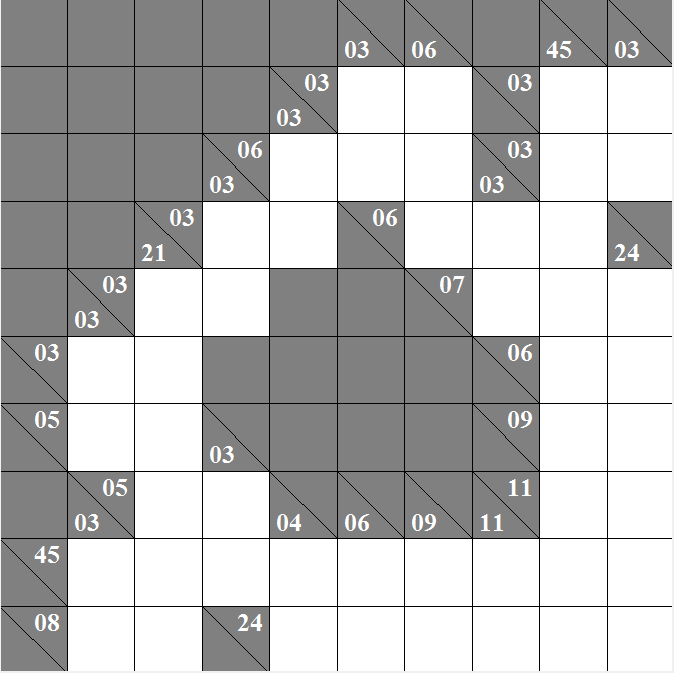
\includegraphics[width = 180pt]{Kakuro_10x10_No.png}
			\caption{Kakuro 10x10}
		\end{figure}

	\end{itemize}

	
	\begin{itemize}
	 \item{\bf Resolver Kakuros:} Corresponde a una de las principales funcionalidades del programa, donde dado un tablero en blanco se intenta lograr una solución final a dicho acertijo, mediante la utilización de algoritmo Backtracking (vuelta atrás) y algoritmos poda, esto con el fin de encontrar una solución de la forma mas acertada posible.
	\end{itemize}

		\begin{figure}[h]
		\centering
		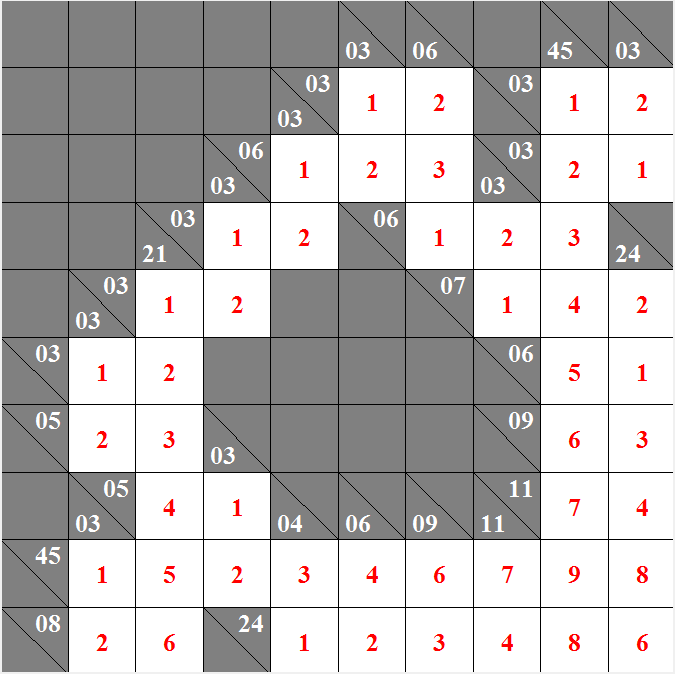
\includegraphics[width = 180pt]{Kakuro_10x10.png}
		\caption{Kakuro 10x10}
		\end{figure}

	\begin{itemize}
	\item{\bf Procesamiento con Hilos:} Se espera además, una forma de "paralelizamiento" para el programa, en el cual mediante el uso de hilos de ejecución, se generen tableros de kakuros, asi como tambien resolverlos.
	\end{itemize}

	\begin{itemize}
	\item{\bf Procesamiento con Forks (Bifurcaciones):} La última forma de "paralelizamiento" esperada, es la ejecución de multiprocesos o bifurcaciones (forks) para, de igual forma, generar y resolver kakuros sin importar el tamaño establecido. Todo esto, con el fin de comprobar la diferencia de los tiempos de ejecución de las activiadas del programa.\\
	
	\end{itemize}



\newpage
\section{Análisis}
En el siguiente apartado se hará el análisis de $O$ Grande de los algoritmos implementados.

	\begin{itemize}
		\item{\bf Poda:} La función Se presenta el análisis de las $Podas$ utilizadas en el algoritmo solución para optimizar su funcionalidad. La primer $poda$ a analizar se encuentra en la función $ProbarPosibilidades$ la cual como se muestra en la figura, muestra un $if$ que compara si una coordenada (ubicación de una casilla blanca) ya se encuentra en la solución final, si se cumple la condición, el valor de esa casilla blanca es restado de la llave y el número de casillas blancas a probar es reducido en 1 y así no tenga que continuar analizando esa casilla. 
		
		
		\begin{figure}[h]
			\centering
			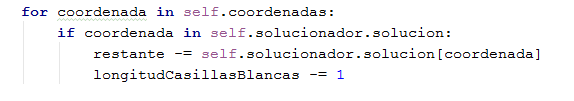
\includegraphics[height= 70pt, width= 280pt]{Poda1.png}
			\caption{Poda 1}
		\end{figure}
	
		La segunda Poda también perteneciente a la función $ProbarPosibilidades$ dada por el $if$ que revisa si la cantidad de casillas blancas es de 2, si se cumple la condicón se llama a la función ObtenerSumas que retornará el vector que conforma el valor de la permutacion restante con 2 y lo añade a la variable combos que almacena las posibles combinaciones de las casillas, esto aprovechando el valor que retorna la variable y así no seguir recorriendo el ciclo $for$ explicado en la primer poda. 
	
		\begin{figure}[h]
			\centering
			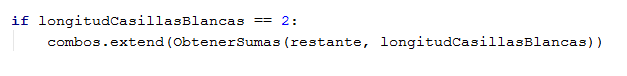
\includegraphics[height= 50pt, width=280pt]{Poda2.png}
			\caption{Poda 2}
		\end{figure}
		
						
	\end{itemize}	

	
	
\newpage
	\begin{itemize}
		\item{\bf Permutación:} Como se muestra en la figura la función $ObtenerSumas$ recibe dos parámetros: el número de la casilla llave y la cantidad de casillas blancas ligadas a este. Esta función se encargará de obtener las posibles combinaciones numéricas para la dada casilla llave. Al iniciar el proceso de la función se compara si la cantidad de casillas blancas es igual a 2, si la condición se cumple, mediante un ciclo $For$ se obtendrán los pares ordenados que sumados consiguen la llave. El orden del $For$ está dado por $O(n)$ donde n representa el número de casilla disminuido por 1. \\En caso contrario de que la primer condición no se cumpla, debido a que la cantidad de casillas es mayor a 2, se realiza un ciclo $For$ el cual hace las posibles sumas para obtener el número llave según la cantidad de casillas blancas. Dicho $For$ se recorre en una llamada recursiva disminuyendo en cada llamada el número de la casilla llave y la cantidad de casillas blancas a tomar en cuenta. Por lo tanto el orden de dicho $For$ está dado por $O(r)$ donde r representa la cantidad de llamadas recursivas iteradas por el ciclo $For$. \\Concluyendo así que el orden total de la función $ObtenerSumas$ conrresponde a $O(n + r)$.
		
		\begin{figure}[h]
			\centering
			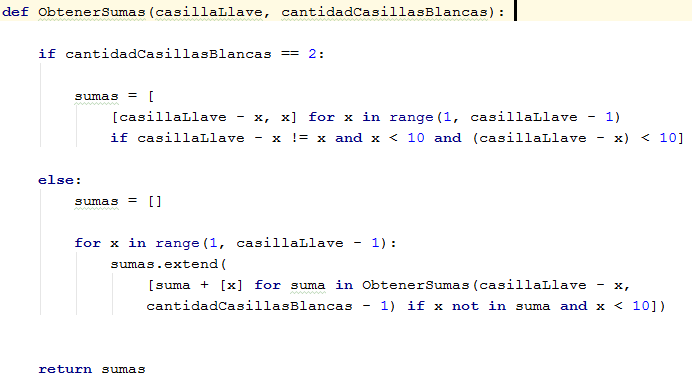
\includegraphics[height= 160pt, width=260pt]{ObtenerSumas.png}
			\caption{Permutación}
		\end{figure}		
		
		\newpage				
		\item{\bf Backtracking:}	De primera instancia, la función de Backtraking recibe tres variables como parametro de entrada, de izquierda a derecha; validos corresponde a las combinaciones posibles de números dado un vector, conjuntoValores el vector con las posibles sumas de las permutaciones que conforman el número llave, por último, recibe un indice cuyo valor inicial es cero, donde su funcionalidad es iterar en el vector $conjuntoValores$, se presentan además, tres asignaciones de variables de las cuales son constantes.

		\begin{figure}[h]
		 	\centering
		 	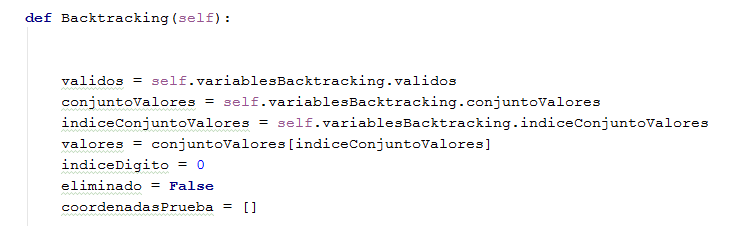
\includegraphics[height= 100pt, width=300pt]{BTVariablesIniciales.png}
		 	\caption{Operaciones Iniciales}
		 \end{figure}
	 
		Seguidamente, sucede un $for$ cuya condición es iterar el vector coordenadas, de la cual se tiene la posición de las casillas blancas asociadas a cada llave del tablero. Dicha condición se realiza $n$ veces. Posteriormente, se realiza un bloque condicional if, donde se comprueba si la actual coordenada del tablero no esta en la solución, dicha condición es constante. 
		
		\begin{figure}[h]
			\centering
			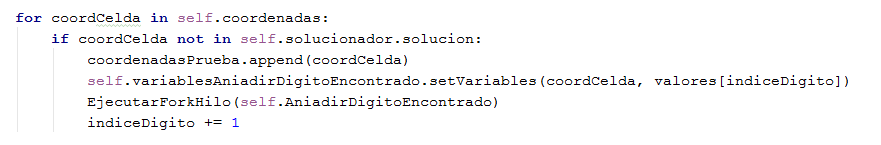
\includegraphics[height= 100pt, width=290pt]{BTFor1.png}
			\caption{Ciclo For 1}
		\end{figure}
		
		Se realiza además, una inserción al vector $coordenadasPrueba$ del cual tambien es operación elemental, en la siguiente linea de código se realiza una llamada a la función $AniadirDigitoEncontrado$ donde recibe tres parametros como entrada; de primera instancia se realiza una asignación de un posíble digito que conforma la casilla llave, al vector solución (solución no final) en la coordenada del tablero que aun no ha sido analizada, lo anterior establecido corresponde a órden constante. Posteriormente, existe un bloque condicional $if$ donde presenta anidados dos condicionales $if$ (separados), de igual manera se consideran como operaciones elementales. Finalizando con la ejecución de la función anteriormente nombrada, se efectua una adición a un vector del cual tambien se considera constante. Una vez finalizada la llamada de la función anterior, se incrementa en uno el indice iterador donde se considera constante.
			
		\begin{figure}[h]
			\centering
			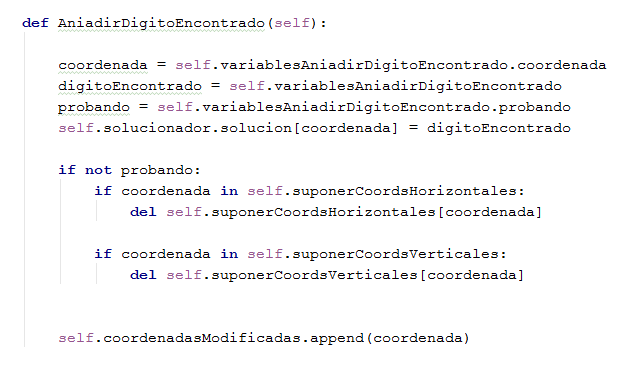
\includegraphics[height= 140pt, width=220pt]{AnadirSolu.png}
			\caption{Función AniadirDigitoEncontrado}
		\end{figure}
	
		Llegado a este punto, se tiene que el órden hasta el momento corresponde a $O(n)$.
		Seguidamente, existe un ciclo $for$ cuya condición consiste en iterar sobre los elementos del vector $coordenadasPrueba$, donde contiene coordenadas que no están en solución (solución no final) y que han sido añadidas como prueba en el bloque condicional $for$ anterior. Mediante el condicional $if$ dentro de ese $for$, se llama a la variable intersecar la cual retorna la celda de posición contraria, es decir, si se envía como parámetro una celda Vertical, la variable retornará esa misma celda pero en su formato Horizontal. Seguidamente utilizando el elemento intersecado por coordenada, se llama a la función $LlenarCeldas$ que recibe el valor booleano True. 
		
		\begin{figure}[h]
			\centering
			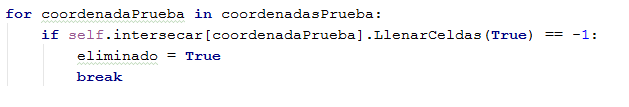
\includegraphics[height= 80pt, width=300pt]{BTFor2.png}
			\caption{Ciclo For 2}
		\end{figure}
	
	
		\begin{figure}[h]
			\centering
			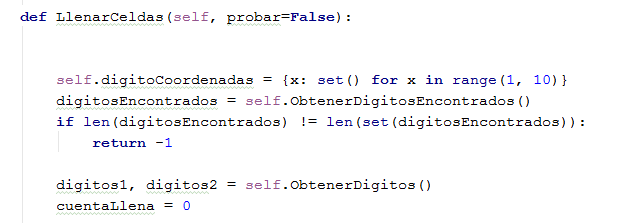
\includegraphics[height= 100pt, width=300pt]{LlenarCeldas1.png}
			\caption{Función LlenarCeldas declaraciones}
		\end{figure}
	
		La función $LlenarCeldas$ toma los datos de la celda indicada y busca los dígitos que ya han sido asignados a las casillas blancas correspondiendes por medio de la función $ObtenerDigitosEncontrados$, la cual retorna una lista con todos los números que forman parte de la solución final. Dicha función funciona mediante un ciclo $for$ que itera sobre todas las coordenadas y las coordenadas pertenecientes a la solución final las une a la lista que retornará. El orden de esa función está dado por $O(n)$ donde $n$ representa todas las coordenadas de las casillas blancas. 
		
		\begin{figure}[h]
			\centering
			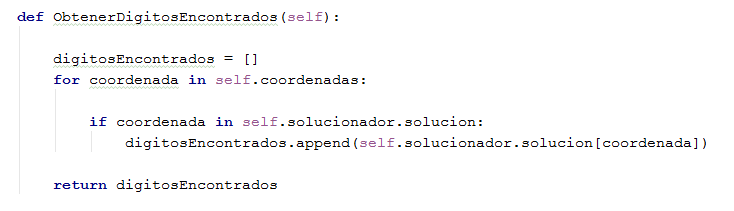
\includegraphics[height= 100pt, width=300pt]{ObtenerDigitosEncontrados.png}
			\caption{Función ObtenerDigitosEncontrados}
		\end{figure}
		
		
		Retomando la función $LlenarCeldas$, esta nuevamente hace la llamada a una función externa, $ObtenerDigitos$ la cual retorna todos los dígitos posibles (excluyendo los dígitos ya encontrados) como una túpla dada por un par ordenado, el cual su primer elemento corresponde al conjunto que contiene la unión de todos los dígitos posibles y su par es el conjunto de dígitos comunes a todas secuencias, que son todas las combinaciones de los posibles números según las casillas blancas formando la casilla llave. Esta función recorre mediante un ciclo $for$ todas las secuencias, y mediante un $if$ revisa si los dígitos encontrados se encuentran en secuencia. Al finalizar le quita a los valores de retorno los dígitos encontrados. Dicha función está dada por $O(o)$ donde $o$ representa la cantidad de vectores en secuencia. 
		
		\begin{figure}[h]
			\centering
			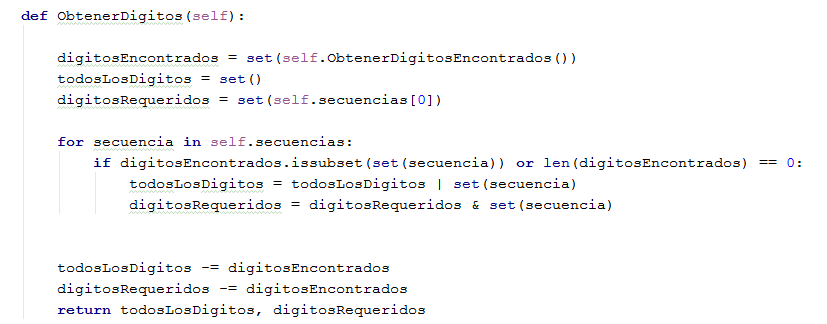
\includegraphics[height= 110pt, width=300pt]{ObtenerDigitos.png}
			\caption{Función ObtenerDigitos}
		\end{figure}
		
		
		Volviendo a $LlenarCeldas$ se recorre en un ciclo $for$ las coordenadas de las casillas blancas ligadas a la llave. Si esa casilla blanca no se encuentra en la solución final se obtienen los vectores con los valores posibles para la posición contraria de esa casilla. Es decir, si se está revisando primeramente una casilla blanca que pertenece a una llave horizontal, por medio de esa llamada se obtendría el valor que puede tomar esa casilla blanca en la perspectiva vertical y se llama nuevamente a $ObtenerDigitos$. 
		Seguidamente se hace la unión de las variables digitos3 y digitos1 los cuales contienen la unión de todos los dígitos posibles que puede almacenar la casilla blanca. Mediante un $if$ se compara si 
		el tamaño del vector digitoComun es de 1, eso significaría que se encontró un posible valor que calza para la matriz vertical y horizontal. Al entrar a este $if$ se llama a la función $AniadirDigitosEncontrados$ que tiene un orden constante. 
		
		\begin{figure}[h]
			\centering
			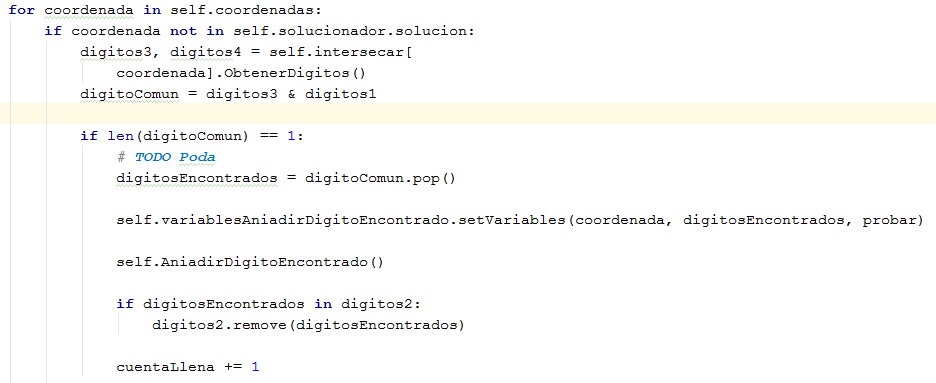
\includegraphics[height= 100pt, width=300pt]{LlenarCeldas2.png}
			\caption{Función LlenarCeldas}
		\end{figure}
	
		\begin{figure}[h]
			\centering
			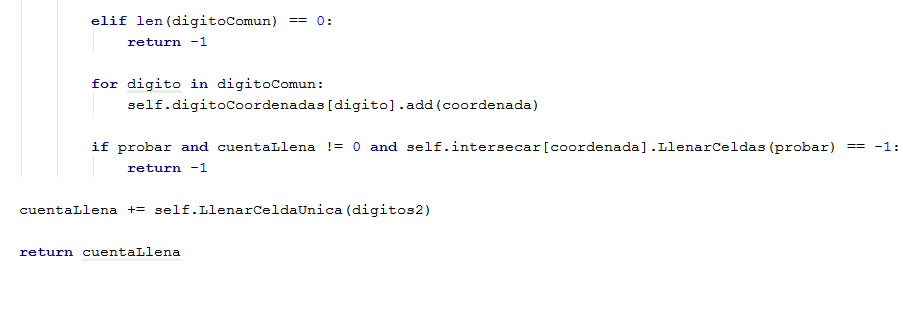
\includegraphics[height= 100pt, width=300pt]{LlenarCeldas3.png}
			\caption{Función LlenarCeldas}
		\end{figure}
		
		Si el $if$ anterior no se cumple, se entra en el condicional $elif$ y compara que si el tamaño del $digitoComun$ es 0, debe retornar -1, es decir, no se encontro valor para la casilla dada.
		Al salir de los condicionales, mediante un $for$ se itera en el vector $digitoComun$ y se añade a la variable que contiene las coordenadas de las casillas blancas. Dicho $for$ tendría un orden de
		$O(d)$ donde $d$ representa la cantidad de valores que contiene el vector $digitoComun$. Seguidamente se muestra un $if$ que si no se ha encontrado un valor para la casilla, se retorna -1.
		Para finalizar se hace el aumento de cuentaLlena llamando la función $LlenarCeldaUnica$, la cual contiene un $for$ que itera sobre los pares ordenados de la variable digitoCoordenadas, seguidamente mediante un $if$ compara si las variables del ciclo $for$ se encuentran en el vector digitosRequeridos, y mediante otro $if$ verifica si la coordenada se encuentra en la solución final para aumentar el contador de números encontrados y hace llamada de la función $AniadirDigitoEncontrado$ con orden constante. Se concluye que la función $LlenarCeldas$ tiene un orden de $O(x[n + o + n(o + d) + q])$, donde $x$ representa la llamada recursiva.
	
		
		Retomando el algoritmo de $Backtracking$, existe un bloque $if$ cuya condición booleana es operación elemental, junto con la añadidura de un elemento al vector. Seguidamente, se presentan dos bloque condicionales $if$ donde se consideran tambien operaciones elementales donde se retorna $True$ si el digito evaluado es solución. Una vez concluido lo anterior, se efectua la llamada a la función $Rehacer$, de la cual deshace un cambio en la solución si un dígito colocado evita que se encuentre una posible solución, en dicha función se presentan dos asignaciones de variables correspondiendo a operaciones elementales, en la siguiente línea se efecta un ciclo $while$ cuya condición de parada es hasta que encuentre la coordenada que causa problemas en la posible solución para posteriormente ser eliminada, por tanto, dicha eliminación se considera operación elemental, y la condición del ciclo $while$ se efectua $m$ veces.
		Continuando con el análisis, existe un bloque condicional $if$, del cual es constante, donde se encarga de realizar la llamada recurviva del algoritmo $i$ veces hasta que se hayan considerado todas las permutaciones posibles. Seguidamente, se presenta otro condicional $if$ donde se considera operación elemental, además de la asignación de una variable posterior al bloque condicional. En la siguiente línea, se presenta un bloque $for$ cuya condición es ser ejecutada hasta que se abarquen las casillas blancas del tablero, es decir $n$ veces, seguidamente existe un condicional considerado constante, además de la llamada a la función $AniadirDigitoEncontrado$ de la cual como se citó anteriormente es constante.
		En conclusión, se tiene que el órden final del algoritmo es $O(i \cdot [n + m(x(n + o + n(o + d) + q)) + m + n])$, donde $i$ representa la llamada recursiva del algoritmo.
		
		Resolviendo la matemática para $f(n)$, se obtiene: \
		
		\begin{center}
			$ f(n) = i \cdot [n + m(x(n + o + n(o + d) + q)) + m + n] $ \
			$ = i \cdot [2n + m(x(n + o + no + nd + q)) + m] $ \
			$ = i \cdot [2n + m((x(o(1 + n) + n(1 + d) + q)) + 1)] $ \
			$ = i \cdot [n + m(x \cdot o \cdot n + nd + q)] $ \
			$ = i \cdot [n + m(n(xo + d) + q)] $ \
			
		\end{center}
		
		$\therefore O(i \cdot [n + m(n(xo + d) + q)]) $ \
		
		
		\begin{figure}[h]
			\centering
			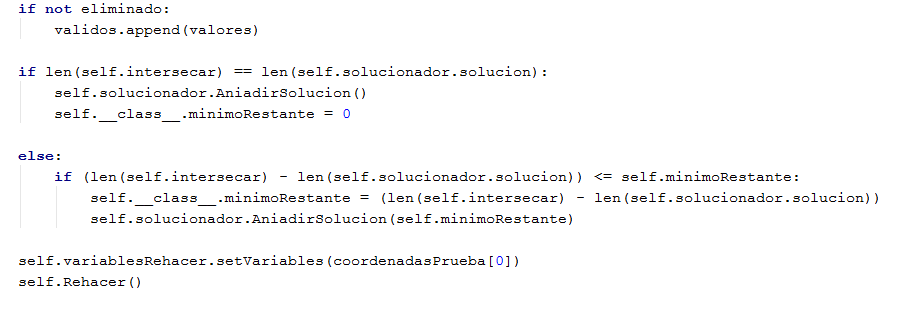
\includegraphics[height= 120pt, width=300pt]{BT3.png}
			\caption{Backtracking}
		\end{figure}
	
		\begin{figure}[h]
			\centering
			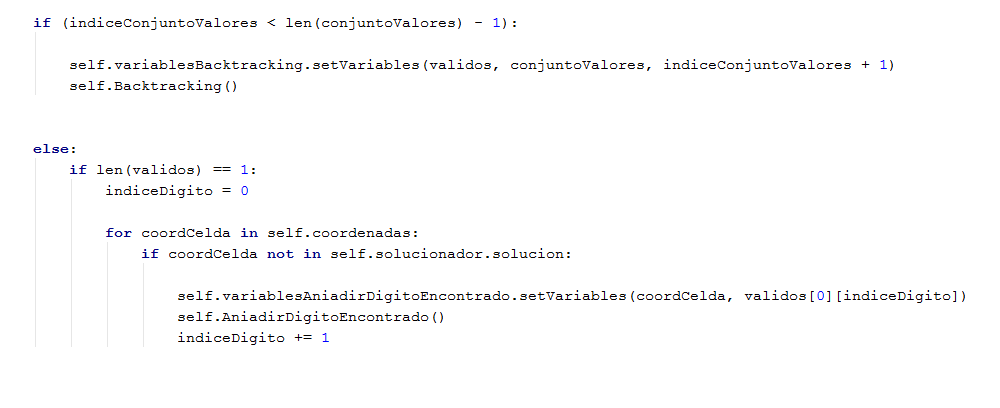
\includegraphics[height= 120pt, width=300pt]{BT4.png}
			\caption{Backtracking}
		\end{figure}
	
	\end{itemize}
		

	
		


\newpage
\section{Experimentos}
A continuación se exponen una serie de experimentos con el programa de Kakuros para conocer su comportamiento a diferentes situaciones. 
\begin{itemize}
	\item{\bf Comparación de duración en segundos:}  \\
	El primer experimento a efectuar consiste en calcular en segundos (s) la duración del programa al momento de solucionar un Kakuro dependiendo del tamaño de la entrada. Para ello se utilizarán Kakuros de tamaño 10x10, 12x12, 15x15, y 20x20. Cabe destacar que la duración es un promedio de aproximadamente 5 Kakuros de la misma dimensión.\\
	Primeramente, para el proceso de solución del Kakuro 10x10, el cual tiene una duración de  2.12 segundos
	
	\begin{figure}[h]
		\centering
		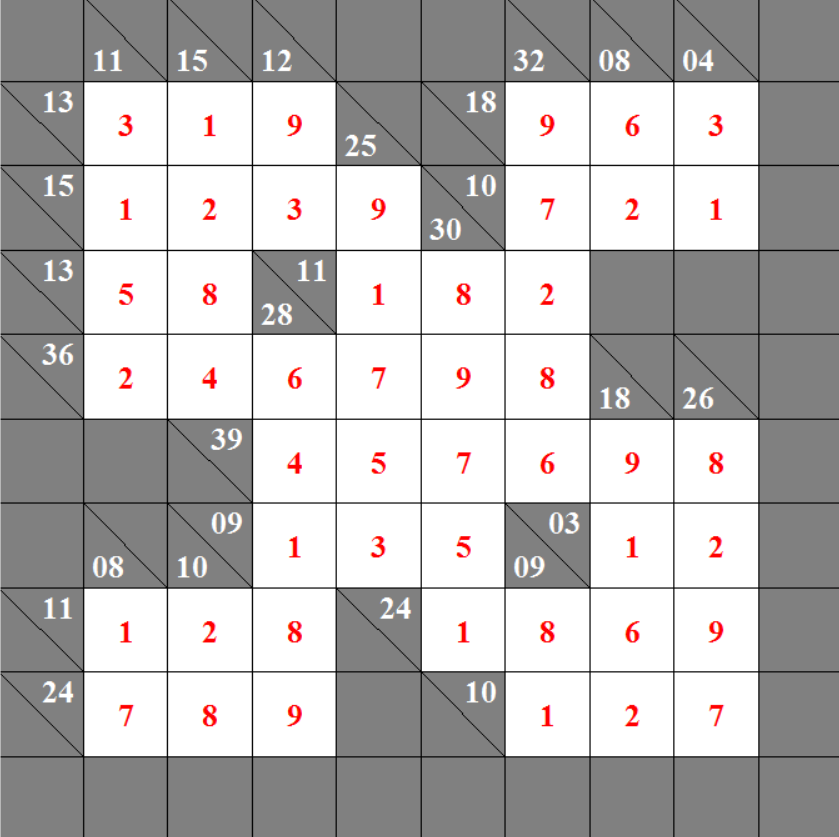
\includegraphics[width=180pt]{ExpKakuro10x10.png}
		\caption{Kakuro 10x10}
	\end{figure}
	
	Para el Kakuro 12x12 su duración corresponde a 2.16 segundos
	
	
	\begin{figure}[h]
		\centering
		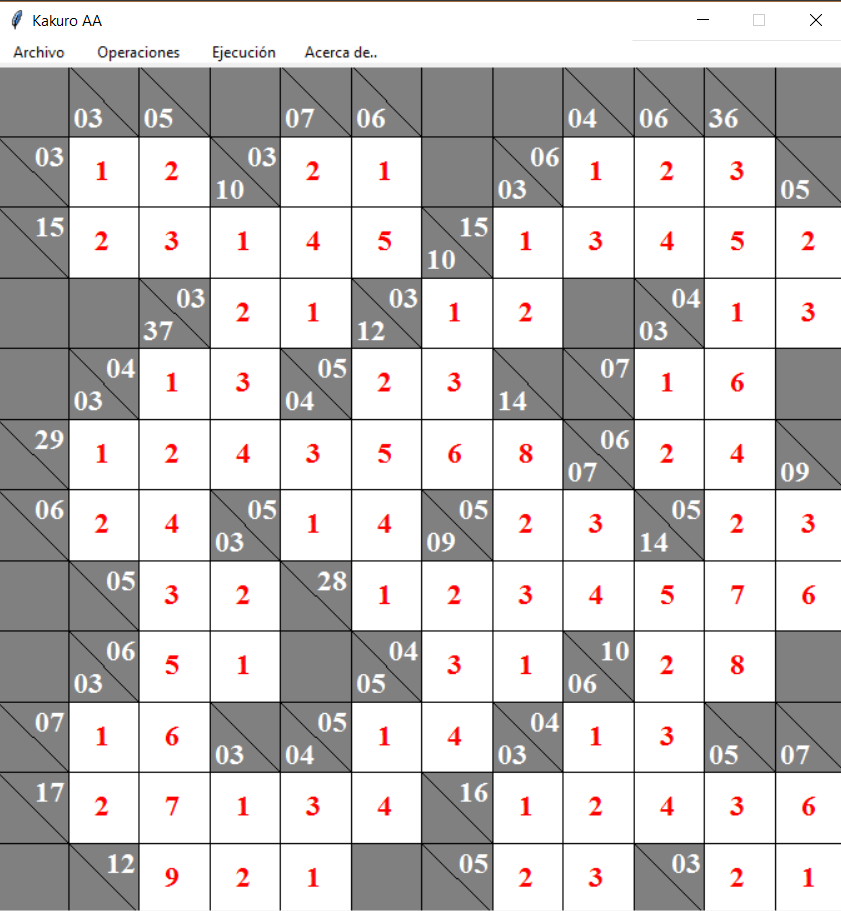
\includegraphics[width=180pt]{ExpKakuro12x12.png}
		\caption{Kakuro 12x12}
	\end{figure}
	
	El Kakuro de dimensión 15x15 el algoritmo tiene una duración de 2.31 segundos
	
	\begin{figure}[h]
		\centering
		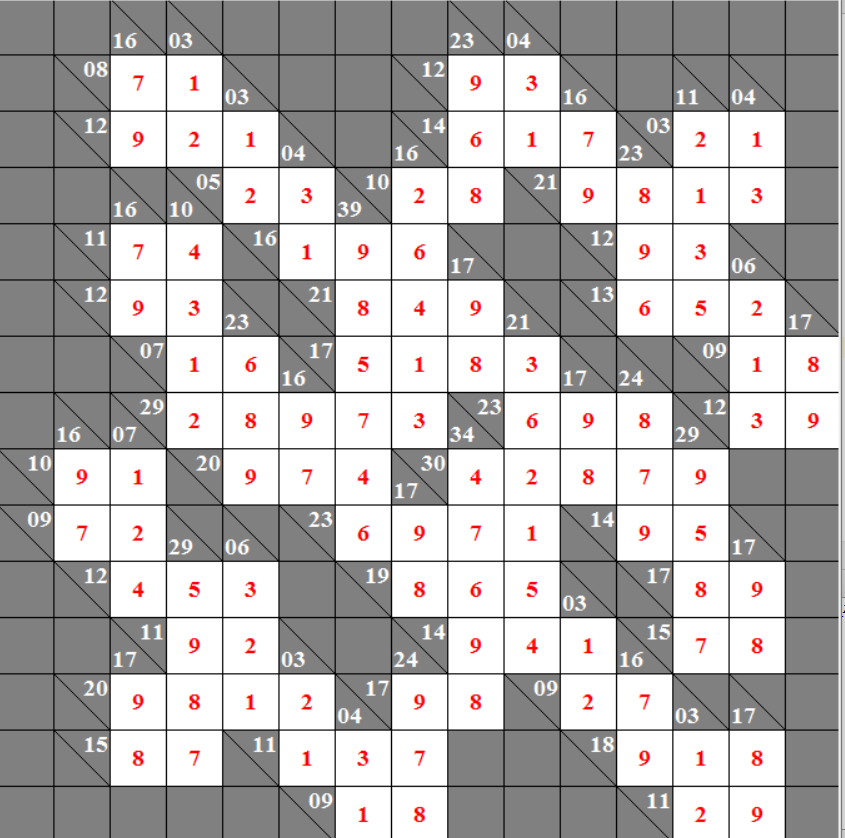
\includegraphics[width=180pt]{ExpKakuro15x15.png}
		\caption{Kakuro 15x15}
	\end{figure}
	
	Para finalizar se hace la ejecución del Kakuro 20x20 el cual tiene una duración de 2.77 segundos
	
	\begin{figure}[h]
		\centering
		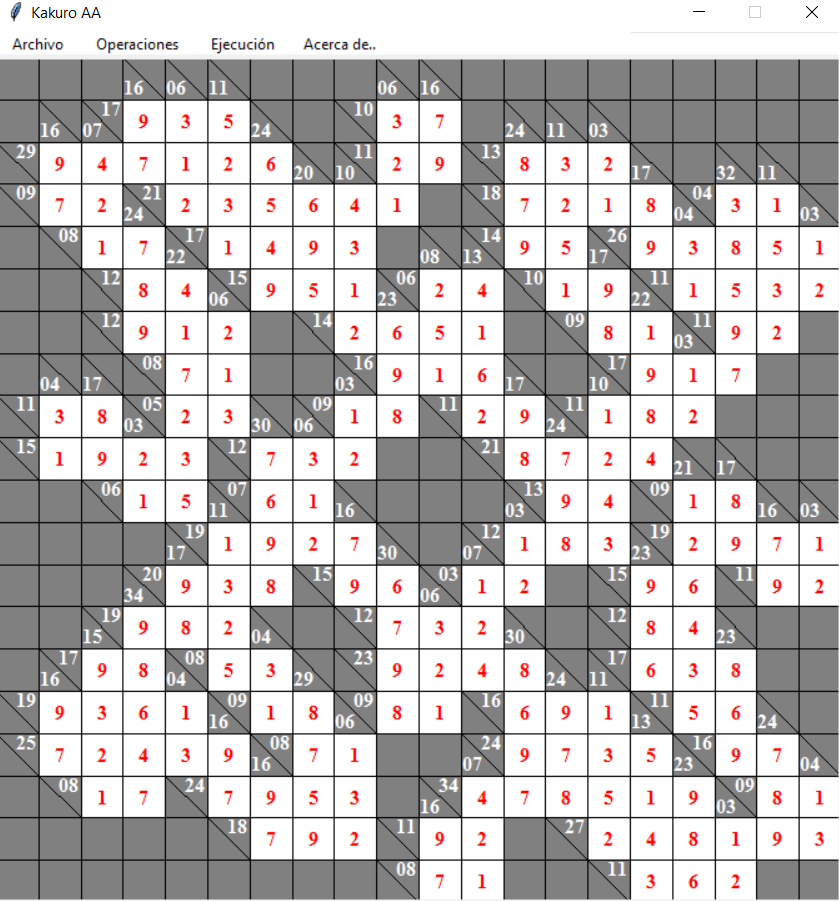
\includegraphics[width=180pt]{ExpKakuro20x20.png}
		\caption{Kakuro 20x20}
	\end{figure}
	
	
	Para concluir, la siguiente gráfica muestra como va creciendo gradualmente la duración del algoritmo al buscar una solución al problema dependiendo de su tamaño de entrada. Como podemos apreciar entre mayor es la dimensión del Kakuro, mayor es la duración del algoritmo buscando una solución a este, esto debido al mayor recorrido de casillas del tablero que debe dedicar el algoritmo.
	
	\begin{figure}[h]
		\centering
		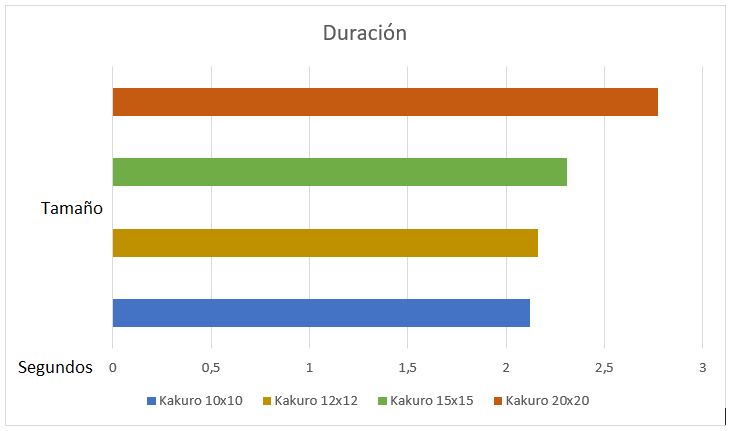
\includegraphics[height= 200pt, width=260pt]{promedioTiempo.png}
		\caption{Comparación de tiempos de ejecución}
	\end{figure}
	
	
	
	\item{\bf Comparación de la duración de la resolución con hilos y sin hilos} \\
	En el siguiente experimento se realiza la comparación de duración entre el algoritmo de resolución de Kakuros implementado con hilos y uno sin paralelización. La duración es un promedio de aproximadamente 5 Kakuros de la misma dimensión. Además para esta comparación se utilizó un solo hizo de ejecución para cada llamada de las funciones implementadas con hilos.\\
	
	Inicialmente se comprueba la duración con hilos de un Kakuro con dimensión 10x10.  este tiene una duración de 2.20 segundos. Para el Kakuro 12x12 este tiene una duración de 2.26 segundos. Seguidamente, comprando el Kakuro 15x15 este muestra una duración de 2.43 segundos. Para finalizar la comprobación, el Kakuro 20x20 tiene una duración de  2.97 segundos.
	
	Analizando el resultado en segundos del algoritmo de resolución de Kakuros con hilos y sin hilos podemos apreciar una diferencia de pocos milisegundos en la duración en tiempo de ejecución, siendo la implementación sin hilos con menor duración. 

	
	
	
\end{itemize}

\newpage
\section{Conclusión}

Dicho proyecto programado, deja como resultado de aprendizaje en el lenguaje de programación Python, un programa generador y solucionador de Kakuros. Se estudió el campo de árboles de búsqueda y el algoritmo de Backtracking que permite devolverse por el árbol si un camino deja de ser prometedor para la solución final. Además se contempló del concepto de Poda, el cual permite obviar caminos y ahorrarse cantidades de recursos en la ejecución de la búsqueda de soluciones. Además se adentró en el concepto de Hilos y Forks los cuales permiten paralizar funciones, es decir, que estas se ejecuten al mismo tiempo y así optimizar la duración de un algoritmo, y se instruyó en la elaboración de estos algoritmos de paralelización. Se realizó la comparación, en segundos, de la duración de la solución de los Kakuros según su tamaño de entrada, en el cual se pudo apreciar que tiene un crecimiento gradual, es decir, entre mayor es la dimensión del kakuro, mayor es la duración del algoritmo al buscar una solución al Kakuro, esto debido a que crece la cantidad de casillas que el algoritmo debe evaluar. En adición a la sección de experimentos se comprobó la duración del algoritmo de solución implementado con hilos, en el cual como en el caso anterior, este aumenta su duración según va aumentado la dimensión del Kakuro a resolver, además se pudo apreciar que la solución sin hilos es unos milisegundos más rápido en comparación al formato de solución con hilos.

\end{document}


